\subsection{Tutorial 2: Pulling on a carbon nanotube}
\label{carbon-nanotube-label}

\begin{figure}
{\centering
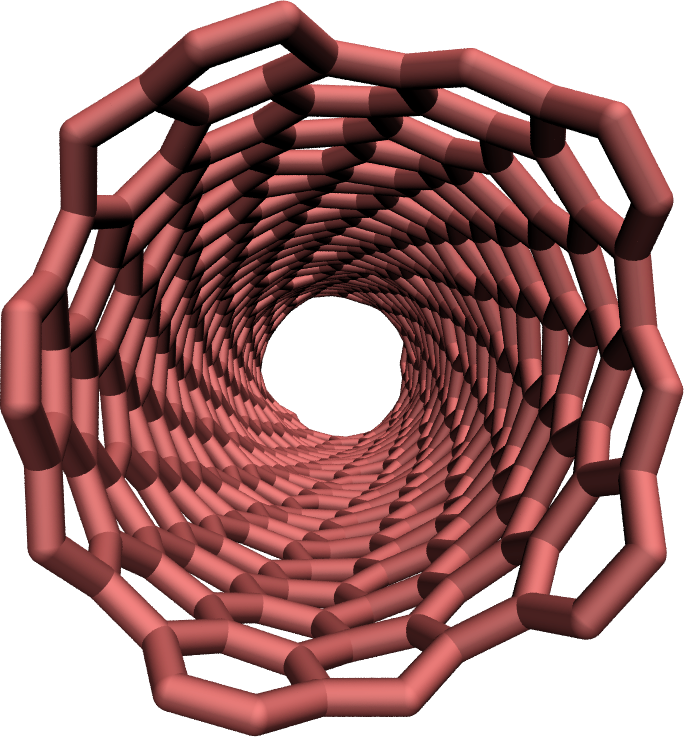
\includegraphics[width=0.55\linewidth]{CNT}
\caption{Snapshot of the carbon nanotube (CNT) made using VMD.}}
\label{fig:CNT}
\end{figure}

\vspace{0.25cm} \noindent The objective of this tutorial is to impose the deformation of a carbon nanotube (CNT) using LAMMPS. In this tutorial, a small carbon nanotube (CNT) is simulated within an empty box using LAMMPS (Fig.\,\ref{fig:CNT}). An external forcing is imposed on the CNT, and its deformation is measured with time. The difference between classical and reactive force fields
is illustrated through this tutorial. With a classical force field, the bonds between atoms are unbreakable. With the reactive force field (named AIREBO \cite{stuart2000reactive}), the breaking of the chemical bonds is possible when the imposed deformation is strong enough.

\subsubsection{Unbreakable bonds}
\noindent With most classical molecular dynamics force fields, the chemical bonds between the atoms are set at the start of the simulation. Regardless of the forces applied to the atoms during the simulations, the bonds remain intact. The bonds between neighbor atoms typically consist of springs with given equilibrium distances $r_0$ and a constant $k_b$: $U_b = k_b \left( r - r_0 \right)^2$.
Additionally, angular and dihedral constraints are usually applied to maintain the relative orientations of neighbor atoms. 

Download directly the CNT topology by clicking \href{https://lammpstutorials.github.io/lammpstutorials-inputs/level1/breaking-a-carbon-nanotube/unbreakable-bonds/cnt_molecular.data}{here}. It was created using VMD and TopoTools \cite{kohlmeyer2017topotools}, and contains information about the positions of the carbon atoms, as well as the
identity of the atoms that are linked by \textit{bonds}, \textit{angles}, \textit{dihedrals},
and \textit{impropers} constraints. Save the \textit{cnt$\_$molecular.data} file
in a folder named \textit{unbreakable-bonds/}.

\paragraph{The LAMMPS input}
Create a new text file within \textit{unbreakable-bonds/} and name it \textit{input.lammps}. Copy the following lines in it:
\begin{verbatim}
variable T equal 300

units real
atom_style molecular
boundary f f f
pair_style lj/cut 14

bond_style harmonic
angle_style harmonic
dihedral_style opls
improper_style harmonic

special_bonds lj 0.0 0.0 0.5

read_data cnt_molecular.data
\end{verbatim}
The chosen unit system is \textit{real} (therefore distances are in Ångstrom, time in femtosecond), the \textit{atom$\_$style} is molecular (therefore atoms are dots that can be bonded with each other), and the boundary conditions are fixed. The boundary conditions do not matter here, as the box boundaries were placed far from the CNT. 

Just like in the previous tutorial, \hyperref[lennard-jones-label]{Lennard Jones fluid}, the pair style is \textit{lj/cut} (i.e. a Lennard-Jones potential with a short-range cutoff) with parameter 14, which means that only the atoms closer than 14 Ångstroms from each other interact through a Lennard-Jones potential. The \textit{bond$\_$style}, \textit{angle$\_$style}, \textit{dihedral$\_$style}, and \textit{improper$\_$style} commands specify the different potentials used to restrain the relative positions of the atoms. For more details about the potentials used here, you can have a look at the LAMMPS website. The \textit{special$\_$bonds} command sets the weighting factors for the Lennard-Jones interaction between atoms directly connected by a bond, separated by two bonds, and separated by three bonds, respectively. The last command, \textit{read$\_$data}, imports the \textit{cnt$\_$molecular.data} file previously generated with VMD, which contains the information about the box size, atom positions, etc.

We need to specify the parameters of both bonded and non-bonded potentials. Here, the parameters are taken from the OPLS-AA (Optimised Potentials for Liquid Simulations-All-Atom) force field \cite{jorgensenDevelopmentTestingOPLS1996}. Create a new text file in the \textit{unbreakable-bonds/} folder and name it \textit{parm.lammps}. Copy the following lines in it:
\begin{verbatim}
pair_coeff 1 1 0.066 3.4
bond_coeff 1 469 1.4
angle_coeff 1 63 120
dihedral_coeff 1 0 7.25 0 0
improper_coeff 1 5 180
\end{verbatim}
The \textit{pair$\_$coeff} command sets the parameters for the non-bonded Lennard-Jones interaction $\epsilon_{11} = 0.066 \, \text{kcal/mol}$ and $\sigma_{11} = 3.4 \, \text{Å}$ for the only type of atom of the simulation; the carbon atom of type 1.  The \textit{bond$\_$coeff} provides the equilibrium distance $r_0= 1.4 \, \text{Å}$ as well as the spring constant $k_b = 469 \, \text{kcal/mol/Å}^2$ for the harmonic potential imposed between two neighboring carbon atoms, where the potential is $U_b = k_b ( r - r_0)^2$. The
\textit{angle$\_$coeff} gives the equilibrium angle $\theta_0$ and constant for the potential between three neighbor atoms :
$U_\theta = k_\theta ( \theta - \theta_0)^2$. The \textit{dihedral$\_$coeff} and \textit{improper$\_$coeff} gives the potential for the constraints between 4 atoms. The file \textit{parm.lammps} is included in the simulation by adding the following line to the \textit{input.lammps} file:
\begin{verbatim}
include parm.lammps
\end{verbatim}


\paragraph{Prepare initial state}
Before starting the molecular dynamics simulation, let us make sure that we start from a clean initial state
by recentering the CNT at the origin (0, 0, 0). In addition, let us make sure that the box boundaries are symmetric with respect to (0, 0, 0), which is not initially the case, as seen in \textit{cnt$\_$molecular.data}:
\begin{verbatim}
-40.000000 40.000000  xlo xhi
-40.000000 40.000000  ylo yhi
-12.130411 67.869589  zlo zhi
\end{verbatim}
Let us recenter the CNT by adding the following lines to \textit{input.lammps}:
\begin{verbatim}
group carbon_atoms type 1
variable carbon_xcm equal -1*xcm(carbon_atoms,x)
variable carbon_ycm equal -1*xcm(carbon_atoms,y)
variable carbon_zcm equal -1*xcm(carbon_atoms,z)
displace_atoms carbon_atoms &
    move ${carbon_xcm} ${carbon_ycm} ${carbon_zcm}
\end{verbatim}
The first command includes all the atoms of type 1 (i.e. all the atoms here) in a group named \textit{carbon$\_$atoms}. 
The 3 variables, \textit{carbon$\_$xcm}, \textit{carbon$\_$ycm}, and \textit{carbon$\_$zcm} are used to measure
the current position of the group \textit{carbon$\_$atoms} along all 3 directions, respectively. Then, the \textit{displace$\_$atoms} 
command move the group \textit{carbon$\_$atoms}, ensuring that its center of mass is located at the origin (0, 0, 0).
Let us also change the box boundaries by adding the following line to \textit{input.lammps}:
\begin{verbatim}
change_box all x final -40 40 y final -40 40 &
    z final -40 40
\end{verbatim}
Such a cleaner and more symmetrical initial state can simplify future data analysis, but won't make any difference to the molecular dynamics.

A displacement will be imposed on the edges of the CNT. To do so, let us isolate the atoms from the two edges and place them into groups named \textit{rtop} and \textit{rbot}, respectively. Add the following lines to \textit{input.lammps}:
\begin{verbatim}
variable zmax equal bound(carbon_atoms,zmax)-0.5
variable zmin equal bound(carbon_atoms,zmin)+0.5
region rtop block INF INF INF INF ${zmax} INF
region rbot block INF INF INF INF INF ${zmin}
region rmid block INF INF INF INF ${zmin} ${zmax}
\end{verbatim}

\noindent The variable $z_\mathrm{max}$ corresponds to the coordinate of the last atoms along $z$ minus 0.5 Ångstroms, and $z_\mathrm{min}$ to the coordinate of the first atoms along $z$ plus 0.5 Ångstroms. Then, 3 regions are defined, and correspond respectively to: $z < z_\mathrm{min}$, (bottom) $z_\mathrm{min} > z > z_\mathrm{max}$ (middle), and $z > z_\mathrm{max}$ (top). Finally, let us define 3 groups of atoms corresponding to the atoms located in each of the 3 regions, respectively, by adding to \textit{input.lammps}:
\begin{verbatim}
group carbon_top region rtop
group carbon_bot region rbot
group carbon_mid region rmid
\end{verbatim}
The atoms of the edges as selected within the \textit{carbon$\_$top} and \textit{carbon$\_$bot} groups can be represented with a different color.

{\color{red}Figure: CNT with atoms from the \textit{carbon$\_$top} and the \textit{carbon$\_$bot} groups are represented with a different color.}

When running a simulation, the number of atoms in each group is printed in the terminal (and in the \textit{log.lammps} file). Always make sure that the number of atoms in each group corresponds to what is expected, just like here:
\begin{verbatim}
10 atoms in group carbon_top
10 atoms in group carbon_bot
680 atoms in group carbon_mid
\end{verbatim}
Finally, let us randomly delete some of the carbon atoms. In order to avoid deleting atoms that are too close to the edges, let us define a new region name \textit{rdel} that starts $2\,Å$ from the CNT edges.
\begin{verbatim}
variable zmax_del equal ${zmax}-2
variable zmin_del equal ${zmin}+2
region rdel block INF INF INF INF &
    ${zmin_del} ${zmax_del}
group rdel region rdel
delete_atoms random fraction 0.02 no rdel &
    NULL 482793 bond yes
\end{verbatim}
The \textit{delete$\_$atoms} command randomly deletes $2\,\%$ of the atoms from the \textit{rdel} group (i.e. about 10 atoms).

{\color{red}Figure: CNT with \textit{10} randomly deleted atoms. }

\paragraph{The molecular dynamics}
Let us specify the thermalization and the dynamics of the system. Add the following lines to \textit{input.lammps}:
\begin{verbatim}
reset_atoms id sort yes
velocity carbon_mid create ${T} 48455 mom yes &
    rot yes
fix mynve all nve
compute Tmid carbon_mid temp
fix myber carbon_mid temp/berendsen ${T} ${T} 100
fix_modify myber temp Tmid
\end{verbatim}
Re-setting the atom ids is necessary before using the \textit{velocity} command, this is done by the \textit{reset$\_$atoms} command.
The \textit{velocity} command gives initial velocities to the atoms of the middle group \textit{carbon$\_$mid}, ensuring an initial temperature of 300 K for these atoms with no overall translational momentum, \textit{mom yes}, nor rotational momentum, \textit{rot yes}.
The \textit{fix nve} is applied to all atoms so that all atom positions are recalculated at every step, and a \textit{Berendsen} thermostat is applied to the atoms of the group \textit{carbon$\_$mid} only \cite{berendsen1984molecular}. The \textit{fix$\_$modify myber} ensures that the \textit{fix Berendsen} uses the temperature of the group \textit{carbon$\_$mid} as an input, instead of the temperature of the whole system. This is necessary to make sure that the frozen edges won't bias the temperature. Note that the atoms
of the edges do not need a thermostat because their motion will be restrained, see below.

To restrain the motion of the atoms at the edges, let us add the following commands to \textit{input.lammps}:
\begin{verbatim}
fix mysf1 carbon_top setforce 0 0 0
fix mysf2 carbon_bot setforce 0 0 0
velocity carbon_top set 0 0 0
velocity carbon_bot set 0 0 0
\end{verbatim}
The two \textit{setforce} commands cancel the forces applied on the atoms of the two edges, respectively. The cancellation of the forces
is done at every step, and along all 3 directions of space, $x$, $y$, and $z$, due to the use of \textit{0 0 0}. The two \textit{velocity} commands set the initial velocities along $x$, $y$, and $z$ to 0 for the atoms of \textit{carbon$\_$top} and \textit{carbon$\_$bot}, respectively. As a consequence of these last four commands, the atoms of the edges will remain immobile during the simulation (or at least they would if no other command was applied to them). The \textit{velocity set} commands impose the velocity of a group of atoms at the start of a run, but does not enforce the velocity during the entire simulation. When \textit{velocity set} is used in combination with \textit{setforce 0 0 0}, as is the case here, the atoms won't feel any force during the entire simulation. According to the Newton equation, no force means no acceleration, meaning that the initial velocity will persist during the entire simulation, thus producing a constant velocity motion.

\paragraph{Data extraction}
Next, in order to measure the strain and stress suffered by the CNT, let us extract the distance $L$ between the two edges as well as the force applied on the edges.
\begin{verbatim}
variable L equal xcm(carbon_top,z)-xcm(carbon_bot,z)
fix at1 all ave/time 10 10 100 v_L &
    file output_cnt_length.dat
fix at2 all ave/time 10 10 100 f_mysf1[1] &
    f_mysf2[1] file output_edge_force.dat
\end{verbatim}
\noindent Let us also add a command to print the atom coordinates in a \textit{lammpstrj} file every 1000 steps.
\begin{verbatim}
dump mydmp all atom 1000 dump.lammpstrj
\end{verbatim}
\noindent Finally, let us check the temperature of the non-frozen group over time by printing it using a \textit{fix ave/time} command:
\begin{verbatim}
fix at3 all ave/time 10 10 100 c_Tmid &
    file output_temperature_middle_group.dat
\end{verbatim}

Let us run a small equilibration step to bring the system to the required temperature before applying any deformation:
\begin{verbatim}
thermo 100
thermo_modify temp Tmid

timestep 1.0
run 5000
\end{verbatim}
With the \textit{thermo$\_$modify} command, we specify to LAMMPS that we want the temperature $T_\mathrm{mid}$ to be printed in
the terminal, not the temperature of the entire system (because of the frozen edges, the temperature of the entire system is not relevant).
Let us impose a constant velocity deformation on the CNT by combining the \textit{velocity set} command with previously defined \textit{fix setforce}. Add the following lines in the \textit{input.lammps} file, right after the last \textit{run 5000} command:
\begin{verbatim}
velocity carbon_top set 0 0 0.0005
velocity carbon_bot set 0 0 -0.0005
run 10000
\end{verbatim}
\noindent The chosen velocity for the deformation is $100\,\text{m/s}$, or $0.001\,\text{Å/fs}$.

{\color{red} Figure: Evolution of the length of the CNT with time. The CNT starts deforming at $t = 5\,\text{ps}$.}

The energy, which can be accessed from the log file, shows a non-linear increase with time once the deformation starts, which is expected from the typical dependency of bond energy with bond distance $U_b = k_b \left( r - r_0 \right)^2$.

{\color{red}Figure: Evolution of the total energy of the system with time. The CNT starts deforming at $t = 5\,\text{ps}$.}

As always, is it important to ensure that the simulation behaves as expected by opening the \textit{dump.lammpstrj} file with VMD.

{\color{red}Figure: CNT before (top) and after (bottom) deformation. See the corresponding \href{https://youtu.be/S05nzreQR18}{video}.}

\subsubsection{Breakable bonds}
When using a classical force field, as we just did, the bonds between atoms are non-breakable. Let us perform a similar simulation, 
but this time using a reactive force field instead, allowing for the bonds to break if the applied deformation is large enough.

\subsection{Input file initialization}
\noindent Create a second folder named \textit{breakable-bonds/} next to \textit{unbreakable-bonds/}, and create a new input file in it called \textit{input.lammps}. Type into input.lammps:
\begin{verbatim}
# Initialisation
variable T equal 300

units metal
atom_style atomic
boundary p p p
pair_style airebo 2.5 1 1
\end{verbatim}
The first difference with the previous part is the unit system, here \textit{metal} instead of \textit{real}, a choice that is imposed by the AIREBO force field. A second difference is the use of the \textit{atom$\_$style atomic} instead of \textit{molecular}, single no explicit bond information is required with AIREBO.

\paragraph{Adapt the topology file}
Since \textit{bond}, \textit{angle}, and \textit{dihedral} do not need to be explicitly set when using AIREBO, some small changes need to be made to the previously generated \textit{.data} file. Duplicate the previous file \textit{cnt$\_$molecular.data}, name the copy \textit{cnt$\_$atom.data}, place it within \textit{breakable-bonds/}. Then, remove all bond, angle, and dihedral information from \textit{cnt$\_$atom.data}. Also, remove the second column of the \textit{Atoms} table, so that the \textit{cnt$\_$atom.data} looks like the following: 
\begin{verbatim}
700 atoms
1 atom types
-40.000000 40.000000  xlo xhi
-40.000000 40.000000  ylo yhi
-12.130411 67.869589  zlo zhi

Masses

1 12.010700 # CA

Atoms # atomic

1 1 5.162323 0.464617 8.843235 # CA CNT
2 1 4.852682 1.821242 9.111212 # CA CNT
(...)
\end{verbatim}
In addition, remove the \textit{Bonds} table that is placed right after the \textit{Atoms} table (near line 743), as well as the \textit{Angles}, \textit{Dihedrals}, and \textit{Impropers} tables. The last lines of the file should look like this:
\begin{verbatim}
(...)
697 1 4.669892 -2.248901 45.824036 # CA CNT
698 1 5.099893 -0.925494 46.092010 # CA CNT
699 1 5.162323 -0.464617 47.431896 # CA CNT
700 1 5.099893 0.925494 47.699871 # CA CNT
\end{verbatim}

\paragraph{Use of AIREBO potential}
Then, let us import the LAMMPS data file, and set the pair coefficients by adding the following lines to \textit{input.lammps}
\begin{verbatim}
# System definition
read_data cnt_atom.data
pair_coeff * * CH.airebo C
\end{verbatim}
Here, there is one single atom type. We impose this type to be carbon by using the letter \textit{C}. The \textit{CH.airebo} file can be
downloaded by clicking \href{https://lammpstutorials.github.io/lammpstutorials-inputs/level1/breaking-a-carbon-nanotube/breakable-bonds/CH.airebo}{here}, and must be placed within the \textit{breakable-bonds/} folder. The rest of the \textit{input.lammps} is very similar to the previous one:

\begin{verbatim}
change_box all x final -40 40 y final -40 40 &
    z final -60 60

group carbon_atoms type 1
variable carbon_xcm equal -1*xcm(carbon_atoms,x)
variable carbon_ycm equal -1*xcm(carbon_atoms,y)
variable carbon_zcm equal -1*xcm(carbon_atoms,z)
displace_atoms carbon_atoms move ${carbon_xcm} &
    ${carbon_ycm} ${carbon_zcm}

variable zmax equal bound(carbon_atoms,zmax)-0.5
variable zmin equal bound(carbon_atoms,zmin)+0.5
region rtop block INF INF INF INF ${zmax} INF
region rbot block INF INF INF INF INF ${zmin}
region rmid block INF INF INF INF ${zmin} ${zmax}

group carbon_top region rtop
group carbon_bot region rbot
group carbon_mid region rmid

variable zmax_del equal ${zmax}-2
variable zmin_del equal ${zmin}+2
region rdel block INF INF INF INF &
    ${zmin_del} ${zmax_del}
group rdel region rdel
delete_atoms random fraction 0.02 no rdel &
    NULL 482793

reset_atoms id sort yes
velocity carbon_mid create ${T} 48455 mom yes &
    rot yes
fix mynve all nve
compute Tmid carbon_mid temp
fix myber carbon_mid temp/berendsen ${T} ${T} 0.1
fix_modify myber temp Tmid
\end{verbatim}
Note that a large distance of 120 Ångstroms was used for the box size along the \textit{z} axis, to allow for larger deformation. In addition, the \textit{change$\_$box} command was placed before the \textit{displace$\_$atoms} to avoid issue with the CNT crossing the edge of the box.

\paragraph{Start the simulation}
Here, let us impose a constant velocity deformation using the atoms of one edge, while maintaining the other edge fix. Do to so,
one needs to cancel the forces (thus the acceleration) on the atoms of the edges using the \textit{setforce} command and set the value of the velocity along the \textit{z} direction. First, as an equilibration step, let us set the velocity to 0 for the atoms of both edges. Let us fully constrain the edges. Add the following lines to LAMMPS:
\begin{verbatim}
fix mysf1 carbon_bot setforce 0 0 0
fix mysf2 carbon_top setforce 0 0 0
velocity carbon_bot set 0 0 0
velocity carbon_top set 0 0 0

variable L equal &
    xcm(carbon_top,z)-xcm(carbon_bot,z)
fix at1 all ave/time 10 10 100 v_L file &
    output_cnt_length.dat
fix at2 all ave/time 10 10 100 f_mysf1[1] &
    f_mysf2[1] file output_edge_force.dat

dump mydmp all atom 1000 dump.lammpstrj

thermo 100
thermo_modify temp Tmid

timestep 0.0005
run 5000
\end{verbatim}
Note the relatively small timestep of $0.0005\,\text{ps}$ used. A reactive force field usually requires a smaller timestep than a classical one. When running \textit{input.lammps} with LAMMPS, you can see that the temperature deviates from the target temperature of $300\,\text{K}$ at the start of the equilibration, but that after a few steps, it reaches the target value.

\paragraph{Launch the deformation}
After equilibration, let us set the velocity to 15 m/s and run for a longer duration than previously. Add the following lines into \textit{input.lammps}:
\begin{verbatim}
# 0.15 A/ps = 15 m/s
velocity carbon_top set 0 0 0.15
run 280000
\end{verbatim}
The CNT should break around step 250000. If not, use a longer run. When looking at the \textit{lammpstrj} file using VMD, you will see
the bonds breaking. Use the \textit{DynamicBonds} representation to properly visualize the bond breaking.

{\color{red}Figure: CNT with broken bonds. See the corresponding \href{https://youtu.be/H2_cjoTcVAM}{video}.}

Looking at the evolution of energy again, one can see that energy increasing with the deformation, before completely relaxing when the CNT finally breaks.

{\color{red}Figure: Evolution of the total energy of the system with time.}
